\clearemptydoublepage
\chapter{Usage Patterns for Off-the-Shelf AI in Model Transformation Tools}

% \begin{abstract} 
%     Model Transformation is a fundamental operation applied to models within Model-Driven Engineering. There are many ways to perform this operation and since the recent advancements of artificial intelligence one can observe a growing use of such tools in model transformation. This paper surveys and classifies existing approaches. We propose a number of composable patterns of use of AI in model transformations, collecting a "phrase book" summarising the state-of-the-art, in a pattern language inspired by existing mega-modeling languages. Our aim is to better understand the impact of AI in model transformation, and explore the viability of unexplored pattern configurations.
    
    
%     \keywords{Model Transformation \and Artificial Intelligence \and Model Driven Engineering}
%     \end{abstract}
%     % \mtodo{add: }


    \section{Introduction}
        % \mttodo{add pictures and tables to the right section} 
        % \mttodo{write a high-level outline for all sections}

        Models and model transformations are a core part of model driven engineering, a well-known paradigm for structured software and system development.
        As the field finds more applications, the modeling and transformation requirements gain in complexity.
        This growth in complexity can come in the form of a satisfaction or optimization problem, for which algorithms and meta-heuristics have been provided by the artificial intelligence community.
        Integrating established artificial intelligence techniques allows engineers to augment their transformations, e.g. with smart rule application or by deducing part of the target model.
        Additionally, machine learning techniques can leverage data to infer complex transformations.

        To understand the modeling processes and tools, particular models can be used, namely mega-models, i.e. diagrams describing modeling artefacts, and their relations.
        Using a language based on common patterns in these diagrams, allows for categorisation of the application of techniques within model transformations. 
        
        % \begin{outline}
        %     \1 MDE / MDE
        %         \2 OMG
        %         \2 EMF
        %     \1 AI
        %         \2 proofs 
        %             \3 logic
        %             \3 sat
        %             \3 csp
        %         \2 natural algorithms
        %             \3 neural nets
        %             \3 evolutionary algorithms
        %     \1 Combining both
        %         \2 simple proofs used for simple transformations
        %             \3 prolog
        %             \3 algorithms
        %         \2 decision problems in transformations
        %             \3 scheduling sub-operations

        %     \1 this paper
        %         \2 structure
        %             \3 Context
        %             \3 Pattern Language
        %             \3 Examples of Patterns
        %                 \4 MT from Learning
        %                 \4 MT from Search
        %                 \4 MT and Search
        %                 \4 MT as Search
        %             \3 Possible Patterns
        %         \2 contrib
        % \end{outline}
        
    % \subsection{Objective of This Paper}
    % \label{ssec:objectives}
        The objective of this paper is to find categories for applications of off-the-shelf artificial intelligence components in model transformations. Two applications can be said to be in the same category, if they fall under the same description. In order to provide concise and unambiguous descriptions of these applications, we propose to create a language, designed for the sole purpose of describing the application of artificial intelligence in the field of model transformations.
        The language can also be used to identify interesting applications which haven't been observed.



        This paper is organised as follows. In \autoref{sec:context} we present the context of study. We define our pattern language in \autoref{sec:patternlanguage} and in \autoref{sec:patterns_in_lit} we apply existing approaches found in the literature. Finally, in \autoref{sec:discussion} and \autoref{sec:conclusion} we discuss future possible patterns and conclude.
        
    \section{Context}
    \label{sec:context}
        
        % \mttodo{not sure that this section is even needed}
        
        \subsection{Transformations and Transformation Tools}
        \label{ssec:context-tranformations}
        \subsubsection{Models, Meta-Models and Transformations}
        \label{sssec:mMMmT}

        Models are a concept widely used. Many kinds of model exist for: weather, economy, information.
        A good model follows a few guidelines: easy, representative, one could say with a goal in mind.
        Models exist in relation to the systems under study they represent. The aim of this representation is to make learning from or building the system easier.
        % \mtreplace{Very simple models can be found among whole numbers representing quantities}{For instance, whole numbers can be considered as very simple models representing quantities}
        For instance, whole numbers can be considered as very simple models representing quantities; Numbers can be manipulated effortlessly compared to the quantities they 
        % \mtdelete{can} 
        represent.

        Meta-Models, are themselves models, however specifically representing a set of models. 
        % \mtnote{A level of abstraction further above the system under study (and similar systems).}{I would delete this, it's not about "level of abstraction"}
        Models within the represented set are said to be conforming models.
        Following the example with whole numbers; while each number is a model, we can represent the set of all numbers with $\mathbb{N}$, and describe the conformity relation as inclusion in this set: $n \in \mathbb{N}$.
        
    \begin{figure}[h]
        \begin{subfigure}[b]{0.3\textwidth}
            \centering
            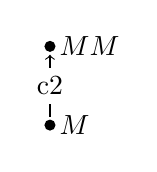
\begin{tikzpicture}
                \coordinate [label=0:{$M$}] (M) at (0,0);
                \coordinate [label=0:{$MM$}]  (MM) at (0,1);
              
                  \fill (M) circle (2pt);
                  \fill (MM) circle (2pt);
                  
                \draw[->, shorten <= 3pt, shorten >= 3pt,] (M) -- (MM) node [midway,fill=white] {c2};
            \end{tikzpicture}
            \caption{Model conforming to Meta-Model}
            \label{fig:c2}
        \end{subfigure}
        \hfill
        \begin{subfigure}[b]{0.3\textwidth}
            \centering
            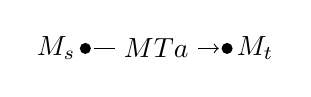
\begin{tikzpicture}
                \coordinate [label=180:{$M_s$}] (M) at (0,0);
                \coordinate [label=0:{$M_t$}]  (MM) at (1.8,0);
            
                \fill (M) circle (2pt);
                \fill (MM) circle (2pt);
                
                \draw[->, shorten <= 3pt, shorten >= 3pt,] (M) -- (MM) node [midway,fill=white] {$MTa$};
            \end{tikzpicture}
            \caption{Transformation applications}
            \label{fig:transformation_application}
        \end{subfigure}
        \hfill
        \begin{subfigure}[b]{0.3\textwidth}
            \centering
            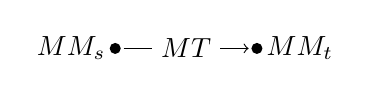
\begin{tikzpicture}
                \coordinate [label=180:{$MM_s$}] (M) at (0,0);
                \coordinate [label=0:{$MM_t$}]  (MM) at (1.8,0);
            
                \fill (M) circle (2pt);
                \fill (MM) circle (2pt);
                
                \draw[->, shorten <= 3pt, shorten >= 3pt,] (M) -- (MM) node [midway,fill=white] {$MT$};
            \end{tikzpicture}
            \caption{Transformation specifications}
            \label{fig:transformation_specification}
        \end{subfigure}
        \hfill
        \caption{Basic patterns of models and transformations}
    \end{figure}

        In \autoref{fig:c2} we can see the first part of the patterns seen in this paper. Depicted are two artefacts $M$ and $MM$, respectively a model and the meta-model it conforms to. The conformity relation, is shown as an arrow labeled \emph{c2} indicating the model $M$ conforms to $MM$.


        Transformations, are the operation applied to models, and are specified at the same level of abstraction as meta-models. In the case of \cite{favre_towards_2005} transformations are akin to whole number functions: sets of relations between antecedent and image, each of those relations is referred to as a \textbf{transformation application}.
        A \textbf{Transformation Specification} is commonly an artefact of a Transformation Framework, such as QVT \cite{kurtev_state_2008} or ATL \cite{jouault_atl_2008} file.
        % \mttodo{citations for the two languages}
        Naturally these are also models; a transformation specification in ATL is a model conforming to the ATL meta-model. This implies that transformation themselves can be source and target of 
        % \mtreplace{higher-order transformations}{transformations (called higher-order transformation)}.
        \emph{higher-order} transformations \cite{paige_use_2009}. 
        % \mttodo{add citation to HOT}
        
        Transformation Specifications, such as ATL or QVT, link between meta-models, generally as a collection of rules matching parts of source and target models.

        % \mtnote{
        In \autoref{fig:transformation_application} and \autoref{fig:transformation_specification} we see again two artefacts, both models or both meta-models (respectively), related by a transformation-application, or a transformation-specification.
        These similar patterns, summarise each a level of abstractions:  between models and between meta-models.
        % }{I would avoid a single definition for both levels, it's confusing and I'm not sure it is correct}
        % alternative proposition
        %In \autoref{fig:function} we see again two artifacts which can be models or meta-models. This patterns represent transformation application (resp. transformation specification) between two models (resp. meta-models).


% \begin{outline}
%     \1 3 concepts built on eachother
%     \2 models of systems \cite{muller_modeling_2009}
%     \2 models of models \cite{favre_foundations_2005-1}
%     \2 transforming models of systems using models of the models \cite{favre_towards_2005}
% \end{outline}

%        note: figures in this paper are also models, specifically mega-models

        These concepts, \emph{modeling} and \emph{transformations}, are applied in many fields, beyond software engineering (the scope of this paper) or even engineering. 
        % \mtodo{endo/exo definition}

        % In software engineering and modeling there are 


%         \subsubsection{MDE}
% % \begin{outline}
% %     \1 application and context
% %     \2 modeling and transforming models in important in engineering
% %     \2 parallel to software engineering using objects
% %     \1 OMG
% %     \2 impact in modeling
% %         \3 UML
% %         \3 OCL
% %     \2 impact in MT
% %         \3 MOF EMF
% % \end{outline}
% % \mttodo{Please remove every occurrence of the word MDE from the paper, it takes us 20 years back. Just use MDE instead}
% The Object Management Group provides standards in Model Driven Engineering applied to software~\cite{bezivin_towards_2001}. After the rise of Object Oriented Programming and \emph{everything as Objects} came the parallel \emph{everything as Models}.

% The Eclipse Foundation is another, providing a range of tools for the Eclipse Modeling Framework.

% They provide Meta-Models, or languages, such as the Unified Modeling Language (UML), of which Class Diagrams (a dialect) is commonly used to represent projects using OOP or Java. OCL, or Object Constraint Language, which extends UML with constraints. MOF or Meta-Object Facility, a Meta-Meta-Model specification.
% For which the Eclipse Provides the Meta-Meta-Model Ecore, an implementation of MOF within the Eclipse Modeling Framework.

% Both MOF and EMF propose frameworks for engineers to build models and transform them. The benefit of the abstraction of meta-meta-model, allows engineers to build their meta-models and subsequently their models. Importantly we can rely on the common structure defined in the meta-meta-model, to describe mappings between elements in source and target meta-model elements. For example, all meta-models in Ecore uses classes and attributes to describe elements, and transformations can map between classes and attributes. Classes and attributes are words described by the Ecore meta-meta-model.


        
        \subsubsection{MDE Transformation Tools}
        There are a wide selection of transformation languages and tools, for models and for graphs. These tools and their use is described the by the core word of the pattern language presented in this paper (see \autoref{sssec:pattern-transfo}). Furthermore, the mega-models used to depict these tools, are some of the earliest mega-models \cite{bezivin_need_2004} and informed how the pattern is depicted in this paper.

        Transformation within engineering, and MDE can have a number of qualities and a number of ways to describe them. First the notion of a transformation's direction in regards to abstraction: transformations can move vertically, from abstract models (e.g. UML) to concrete ones (e.g. Java) or the other way around, and transformations can move horizontally at the same level of abstraction (Java to C++).
        Another important aspect of transformations is the relation between the source and target meta-models: in cases where they are different, we talk of Exogenous Transformations (UML to Java, Java to C++) allowing use to move between contexts, other wise we talk of Endogenous Transformations (Java to Java) which generally allows for tasks like optimisations, refactoring, etc.
         
        Notable transformation tools of MDE found in this paper are QVT \cite{petter_solving_2009}, ATL \cite{lecalvar_coupling_2021,le_calvar_toward_2019}, Viatra \cite{horvath_dynamic_2012}, JESS \cite{faunes_generating_2012,faunes_genetic-programming_2013} and Hensin \cite{eisenberg_towards_2021,fleck_marrying_2015}. They each provide different concepts for specifying transformations, such as conditions for rule application, or graph representations and matching. Aside from transformation languages and engines, OCL is commonly used: it provides a query language to map meta-model classes and attributes, and can provide verification of the models and transformations. 

        % \mtodo{OCL query language to map between meta-models}

        % \begin{outline}
        %     \1 Many Transformations lagnuages
        %     \1 represented in \autoref{fig:transfo}
        %     \1 Two main here are QVT and ATL
        %         \2 both target languages for MTBE
        %     \1 QVT
        %         \2 OMG/MOF
        %         \2 %\cite{}
        %     \1 ATL
        %         \2 EMF
        %         \2 \cite{paige_model_2009,strommer_model_2008}
        %     \1 Others
        %         \2 Henshin \cite{eisenberg_towards_2021}
        %         \2
        % \end{outline}

% \begin{table}[!h]
%     \centering
%     \begin{tabular}{|c|c|c|c|}
%     \hline
%         Tool/Qualities & MT & GT & Incremental\\
%     \hline
%         ATL &X&&X \\
%     \hline
%         QVT &X&& \\
%     \hline
%         CoqTL &X&& \\
%     \hline
%         Viatra & &X&X \\
%     \hline
%     \end{tabular}
%     \caption{Transformation Tools and their Qualities}
%     \label{tab:TransfoTools}
% \end{table}

        
        % \subsection{Mega-Model Meta-Models}
        % % how we got to the patterns
        % \subsubsection{MegaL and Favre et al.}
        % \subsubsection{Muller et al.}
        % \subsubsection{T-Core}
        
        \subsection{Off-the-Shelf AIs}
        \label{ssec:offtheshelfAI}

        The definition of AI is fairly wide and what people picture when faced with the term has evolved over time. Today, Neural Networks and Evolutionary Algorithms, are first to mind, allowing us to find solutions to complex problems within reasonable effort, time and accuracy. These contrast with more mature AI tools based on logical induction or satisfiability which while often requiring more effort and time, can achieve exact and explainable solutions.

        We will call AI, \emph{a generalised approach which can solve many problems}. A \textbf{Problem Specification} is the encoding of the problem in a form suitable as input to the AI tool. Concretely in this paper we consider the following families of AI tools:

        % In a similar way as to how NP problems can be translated into SAT, a wide array of problems can be modeled in ways to reuse "solving tools". 
        
        
        % \begin{outline}
        %     % \1 GA 
        %     %     \2 genetic algorithm
        %     %     \2 solutions compete to survive
        %     %     \2 and are mixed to create new solutions
        %     % \1 PSO 
        %     %     \2 Particle swarm algorithms
        %     %     \2 models birds flocking
        %     % \1 SA 
        %     %     \2 Simulated annealing
        %     %     \2 metaheuristic to approximate global optimization in a large search space for an optimization problem.
        %     % \1 Logic 
        %     %     \2 prolog, asp
        %     % \1 CSP 
        %     %     \2 Choco, Cassowary
        %     % \1 Q-Learning \cite{eisenberg_towards_2021,ludovico_model_2020}
        %     \1 Neural Net LSTM \cite{burgueno_lstm-based_2019}
        %     % \1 Ad-Hoc algorithm for MTBE? \cite{paige_model_2009}
        % \end{outline}

        \textbf{Logic Programming} (LP) \cite{petter_solving_2009,balogh_model_2009,kessentini_model_2008,kessentini_generating_2010,kessentini_search-based_2012} has been a mainstay of AI since the beginning of the field. Notable tools from this field are Prolog and ASP, providing simple yet expressive languages to define NP class problems, and a variety of algorithms to find solutions.
        Problems and Solutions are encoded using axioms and rules of inference, allowing to search for solutions and prove them.
        
        Similarly, \textbf{Constraint Programming} (CP or CSP) \cite{le_calvar_toward_2019,petter_solving_2009,horvath_dynamic_2012} provides simple languages to model complex problems, and additional algorithms and heuristics to search for solutions.
        Constraints can be satisfied, by searching for solutions.
        Problems are modeled using variables which can be numeric, sets, graphs, etc.., depending on the solver, and constraints between these variables such as: equality or inferiority between numbers, or inclusion for sets.

        % The notion of constraints serve another use, to express evaluation functions.

        \textbf{Genetic Algorithms} (GA) \cite{faunes_generating_2012,fatiregun_evolving_2004,fatiregun_search_2003,cooper_optimizing_1999,kulkarni_fast_nodate} inspired by the mechanism of genetic evolution and natural selections, encode the problem and it's solutions in an evaluation function and a population of genomes, each individual genome being a possible solution.
        The genomes with the best value are selected to be mutated and mixed, providing a form of local search.

        \textbf{Particle Swarm Optimisation} (PSO) \cite{kessentini_model_2008,kessentini_generating_2010,kessentini_search-based_2012} is another algorithm inspired by nature has found application in model transformations, itself a model of flocking birds. Like GA uses a population representing solutions, except solutions are encoded as positions in space, searching a position of high value.

        \textbf{Simulated Annealing} (SA) \cite{kessentini_generating_2010,kessentini_search-based_2012} provides a meta-heuristic for global search (as opposed to GA or PSO), again by modeling a natural process: the heat treatment of metals, with the aim to \emph{crystallise} optimal solutions. Similarly to PSO, solutions are expressed as positions in space.

        \textbf{Q-Learning} (QL) \cite{eisenberg_towards_2021,ludovico_model_2020} is a method to estimate the value of actions which can be performed given a certain state. In the context of model transformations, this allows us to represent models as states and transformations as actions, and explore the eventual values of transformation actions.

        \textbf{Neural Networks} (NN) \cite{burgueno_lstm-based_2019} are one of the AI getting the most attention today, specifically Long Short-Term Memory (LSTM) structures which show great promise with their application in large language models such as GPT. This version of neural networks, as do others, use a vectorised representation as input and output connected by a network of neurons.
        
        % \subsubsection{Exact Resolution}
        % csp, sat, logic
        % \begin{outline}
        %         \1 logic
        %         \1 sat
        %         \1 csp
        % \end{outline}
        % \subsubsection{not-exact resolution}
        % \begin{outline}
        %     \1 Neural Nets
        %         \2 LSTM encoder/decoder
        % \end{outline}
        
        

        
    \section{Pattern Language}
    \label{sec:patternlanguage}
    % \begin{outline}
    %     \1 Two directions in pattern language
    %         \2 left to right: target transformation direction
    %         \2 top to bottom: higher-order transformations to target transformation
    %     \1 can be expressed as a Context Sensitive Grammar of relations

    % \end{outline}

        In brief terms, to give a first intuition on our understanding of pattern languages: a set of patterns which can be tiled to make bigger patterns, can be described as a language. A simple pattern similar to the one proposed by this paper, is portrayed in \autoref{fig:squarepattern}, along with the rule that two patterns, can by placed side-by-side if their touching shapes are the same colour. The square title it's self is a pattern of coloured triangles, and by tiling the patterns together we can make larger patterns.
            

        \begin{figure}
            \centering
            \begin{minipage}{.35\textwidth}
                \centering
                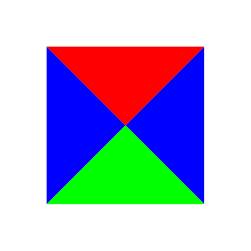
\begin{tikzpicture}
                    \coordinate [label=-100:{}]  (SM) at (0,0);
                    \coordinate [label=-80:{}] (TM) at (2,0);
                    \coordinate (M) at (1,1);
                    \coordinate [label=100:{}]  (SMM) at (0,2);
                    \coordinate [label=80:{}]  (TMM) at (2,2);          

                    \fill[blue,ultra thick] (M) -- (SM) -- (SMM);
                    \fill[blue,ultra thick] (M) -- (TM) -- (TMM);
                    \fill[red,ultra thick] (M) -- (TMM) -- (SMM);
                    \fill[green,ultra thick] (M) -- (SM) -- (TM);
                \end{tikzpicture}
                \caption{Example pattern language tile}
                \label{fig:squarepattern}
            \end{minipage}\hfill
            \begin{minipage}{.60\textwidth}
                \centering
                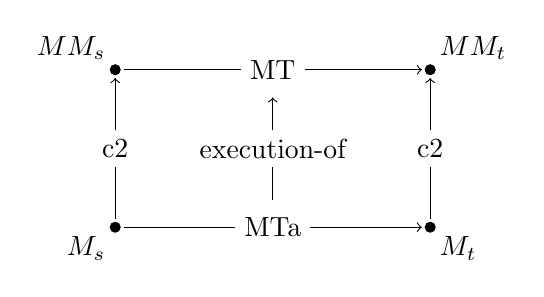
\begin{tikzpicture}
                    \coordinate [label=-100:{$M_s$}]  (SM) at (0,0);
                    \coordinate [label=-80:{$M_t$}] (TM) at (4,0);
                    \coordinate (M2M) at (2,0);
                    
                    \coordinate [label=100:{$MM_s$}]  (SMM) at (0,2);
                    \coordinate [label=80:{$MM_t$}]  (TMM) at (4,2);
                    \coordinate (MM2MM) at (2,2);
                    
                        \fill (SM) circle (2pt);
                        \fill (TM) circle (2pt);
                        \fill (SMM) circle (2pt);
                        \fill (TMM) circle (2pt);
                    
                    \draw[->, shorten <= 3pt, shorten >= 3pt] (SM) -- (TM) node [midway,fill=white] {MTa};
                    \draw[->, shorten <= 3pt, shorten >= 3pt] (SMM) -- (TMM) node [midway,fill=white] {MT};
                    \draw[->, shorten <= 3pt, shorten >= 3pt,] (SM) -- (SMM) node [midway,fill=white] {c2};
                    \draw[->, shorten <= 3pt, shorten >= 3pt] (TM) -- (TMM)node [midway,fill=white] {c2};
            
                    \draw[->, shorten <= 10pt, shorten >= 10pt,] (M2M) -- (MM2MM) node [midway,fill=white] {execution-of};
                \end{tikzpicture}
                \caption{Transformation Pattern}
                \label{fig:transfo}
            \end{minipage}
        \end{figure}


        Our patterns share similar structure to this example, however require more nuance than the colors proposed here and additional structural rules for the larger pattern, and hence more elaborate rules such as: there must be a continuous chain of tiles connected along their blue sides, where none of the greens sides have a neighbour, but to motivate and understand this rule, we need to understand the semantics of our patterns.

        In this paper, patterns used as tiles are mega-models depicting relations between models. Said mega-models are composites of \autoref{fig:c2}, \autoref{fig:transformation_application} and \autoref{fig:transformation_specification} (which serve the role of the letters for the words of our language). The mega-models, or words of the language proposed here, have a similar structure to \autoref{fig:squarepattern}: the blue areas housing mega-models of conformant-models and their meta-models as seen in \autoref{fig:c2}, the red and green areas, holding respectively mega-models or models related by transformation specification \autoref{fig:transformation_specification} or application \autoref{fig:transformation_application}.

        The pattern makes use of two dimensions, patterns can be placed side-by-side from left to right, or placed above patterns. The primary dimension is drawn between a source and target model, made up of a continuous chain of transformations-like operations.
        The line from source to target model must remain unbroken and the lowest side of the composed pattern.
        Above transformations specifications, using secondary dimension: higher-order transformations can be chained. Allowing to create or augment the transformations applied.
        % \mtodo{left-right is entwinned with time}
        
        We propose this pattern language over mega-models to help identify and categorise how artificial intelligence has been applied to model transformations. The vocabulary is made up of simple patterns representing the processes performed by transformation technologies and AIs, while the grammar describes how these actions and patterns can be chained and composed.
        
        To develop this language, cases of artificial intelligence in model transformations \cite{lecalvar_coupling_2021,burgueno_lstm-based_2019,petter_solving_2009,eisenberg_towards_2021} were mega-modeled using concepts from established mega-modeling languages \cite{favre_towards_2005,muller_modeling_2012}, allowing the identifications and isolation of common patterns. 

% \mtodo{Fig 1 and 2 are the letters in the words}
        
        \subsection{Words of the Pattern Language}

        We have three core patterns - words in the language - found in the literature. Two of these words, \emph{AI Learning} and \emph{AI Processing} specifically describe the use of AI in the model transformation process. Both of these processes can be implemented by a variety of the \emph{off-the-shelf} AI suggested in \autoref{ssec:offtheshelfAI}.
        These are in addition to the core word of our field: \emph{Transformation}.
        
        \label{ssec:pattern-vocab}
        \subsubsection{Transformation}
        \label{sssec:pattern-transfo}

        The core pattern for this paper, described in \autoref{fig:transfo}, is naturally that of transformations. In our context, a transformation implies a collection of artefacts and relations.  
        
        
        % \begin{outline}
        %     \1 first pattern is Transformation in it's most general form
        %         \2 in-out relation between two meta-models implying
        %         \2 in-out relations between conforming-models
        %         \2 and the implied conformity relations
        %     \1 in \ref{fig:transfo} singular model is transformed
        %         \2 MTs define sets of MTa
        %         \2 could/should replace $M_s$ with the singleton $\{M_s\}$
        %         \2 but to better identify the target transformation we'll use the single model, and single application, along the bottom of the pattern
        % \end{outline}
        In \autoref{fig:transfo} we can see two models and the meta-models they each conform to. On the left source models, on the right target models. Between the meta-models the transformation specification $MT$ and between the models a transformation application $MTa$.
        Additionally in this mega-model is represented the relation between definition and application, named here \emph{execution of}.

        This pattern is representative of standard transformation tools such as ATL or QVT, but also represents other tools and algorithms which can serve the purpose of transformations, such as general programming languages, logic programming languages, or even neural networks, or even whole transformations processes including a variety of these or \emph{AI Processes} outside of the focus of the pattern.


        \subsubsection{AI Learning}
        \label{sssec:pattern-learn}

        This pattern mirrors the transformation pattern; in the previous pattern, the applications came as executions of the definition, in this pattern the definition is derived from applications or generally, mappings between sets of example source and target models. In the diagram, the direction of the arrow between Specification $MT$ and Application $MTa$ has been inverted.
        In our scope the responsibility of these higher-order transformations is conferred to artificial intelligence, in the hopes of allowing the easy definition of complex transformations.
        
        In \autoref{fig:learn} we find a similar pattern to transformation, at the top between meta-models we have a transformation specification $MT$. However at the model level-of-abstraction, the lower side of the pattern, we predominantly have sets of models and mappings between them, as many machine learning techniques rely on large amounts of example models, or in the case of reinforcing a transformation: prior executions. These sets ${M_s}$ and ${M_t}$ are depicted as conforming to their respective meta-models, which is to mean each model of either set is a conformant-model, and between them a form of mapping ${MTa}$, which is to say a set of source-target relations, like a function.

        This figure is oriented with higher-levels of abstraction (meta-models) at the top, like with \autoref{fig:transfo} and \autoref{fig:search}, however when in use, the pattern is flipped vertically. That way the vertical dimension of the diagram represents the process in place to generate an artifact that can substitute a transformation specification.
        
        % \mtodo{finish describing picture, and point out the difference, warn the pattern is upside down} 
        In our examples the resulting transformation specification can take on a few forms, as previously mentioned for the transformation mega-model, notable examples will be traditional definitions in ATL or JESS \cite{faunes_generating_2012,faunes_genetic-programming_2013}, blackbox functions like neural networks~\cite{burgueno_lstm-based_2019} or an augmented version of a previous definition~\cite{eisenberg_towards_2021,fleck_marrying_2015}.
        % \begin{outline}
        %     % \1 \{MTa\} is a mapping
        %     % \1 MT can be a few things
        %     %     \2 a QVT or ATL definition \cite{?}
        %     %     \2 augmented MT 
        %     %     \2 a neural network 
        %     %     \2 \cite{}
        % \end{outline}


            \begin{figure}
                \centering
                \begin{minipage}[t]{.45\textwidth}
                    \centering
                    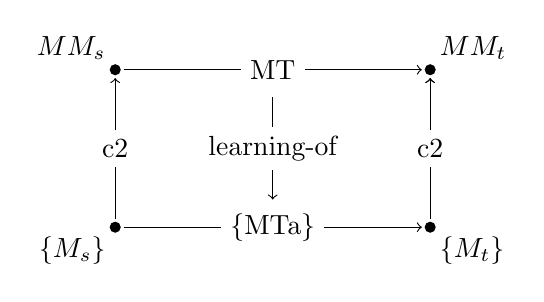
\begin{tikzpicture}
                        \coordinate [label=100:{$MM_s$}]  (SMM) at (0,2);
                        \coordinate [label=80:{$MM_t$}] (TMM) at (4,2);
                        \coordinate (MM2MM) at (2,2);
                    
                        \coordinate [label=-100:{$\{M_s\}$}]  (SM) at (0,0);
                        \coordinate [label=-80:{$\{M_t\}$}]  (TM) at (4,0);
                        \coordinate (M2M) at (2,0);
                    
                        \fill (SM) circle (2pt);
                        \fill (TM) circle (2pt);
                        \fill (SMM) circle (2pt);
                        \fill (TMM) circle (2pt);
                    
                        \draw[->, shorten <= 3pt, shorten >= 3pt] (SMM) -- (TMM) node [midway,fill=white] {MT};
                        \draw[->, shorten <= 3pt, shorten >= 3pt] (SM) -- (TM) node [midway,fill=white] {\{MTa\}};
                        \draw[->, shorten <= 3pt, shorten >= 3pt,] (SM) -- (SMM) node [midway,fill=white] {c2};
                        \draw[->, shorten <= 3pt, shorten >= 3pt] (TM) -- (TMM)node [midway,fill=white] {c2};
                        \draw[->, shorten <= 3pt, shorten >= 3pt] (TM) -- (TMM)node [midway,fill=white] {c2};
                    
                        \draw[->, shorten <= 10pt, shorten >= 10pt,] (MM2MM) -- (M2M) node [midway,fill=white] {learning-of};
                    \end{tikzpicture}
                    \caption{Transformation Learning Pattern}
                    \label{fig:learn}
                \end{minipage}\hfill
                \begin{minipage}[t]{.45\textwidth}
                    \centering
                    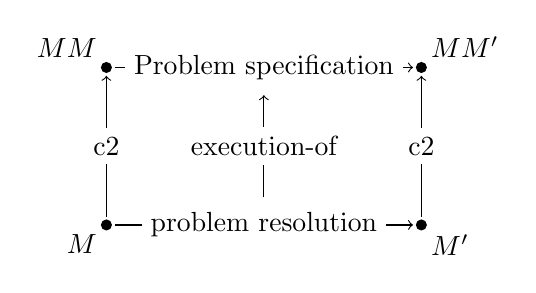
\begin{tikzpicture}
                        \coordinate [label=-100:{$M$}]  (SM) at (0,0);
                        \coordinate [label=-80:{$M'$}] (TM) at (4,0);
                        \coordinate (M2M) at (2,0);
                      
                        \coordinate [label=100:{$MM$}]  (SMM) at (0,2);
                        \coordinate [label=80:{$MM'$}]  (TMM) at (4,2);
                        \coordinate (MM2MM) at (2,2);
                      
                        \fill (SM) circle (2pt);
                        \fill (TM) circle (2pt);
                        \fill (SMM) circle (2pt);
                        \fill (TMM) circle (2pt);
                        
                        \draw[->, shorten <= 3pt, shorten >= 3pt] (SM) -- (TM) node [midway,fill=white] {problem resolution};
                        \draw[->, shorten <= 3pt, shorten >= 3pt] (SMM) -- (TMM) node [midway,fill=white] {Problem specification};
                        \draw[->, shorten <= 3pt, shorten >= 3pt,] (SM) -- (SMM) node [midway,fill=white] {c2};
                        \draw[->, shorten <= 3pt, shorten >= 3pt] (TM) -- (TMM)node [midway,fill=white] {c2};
                      
                        \draw[->, shorten <= 10pt, shorten >= 10pt,] (M2M) -- (MM2MM) node [midway,fill=white] {execution-of};
                      \end{tikzpicture}
                    \caption{Problem Solving Pattern}
                    \label{fig:search}
                \end{minipage}
            \end{figure}


        \subsubsection{AI Processing}
        \label{sssec:pattern-search}

        % This pattern is an alternative to the standard one of model transformations, it can be seen as performing a similar function to transformations, taking models of potential attribute values returning models of possible attribute values. 
        % Models in constrains and logic are expressed in their own languages (a different technical space?), outside of the MDE framework, and doesn't usually benefit from the vocabulary of Endo/Exogenous or Vertical/Horizontal Transformations.

        % Logic language can be used to make meta-models, and inference rules can map between them, while constraint models can allow us to make prototype models, skeletons with possible attributes, refined.
        
        % Generally model transformation tools allow to map between meta-models, but without the provision to find solutions that may be described in OCL. \mtodo{link between meta-models and MOF, and constraints and OCL}

        % \begin{outline}
        %     \1 Two possible versions of the pattern
        %         \2 Solver alone (here)
        %         \2 Solver + MT (execution merge rule)
        %     \1 Solver alone
        %         \2 off the shelf solvers aren't plug and play with MT afaik
        %         \2 generally endo-trasfo
        %     \1 Sover+MT
        %         \2 can be exo-trasfo
        %         \2 logic transfo and solve
        % \end{outline}
        

        In \autoref{fig:search} we can see two models $M$ and $M'$ which each conform to their respective meta-models $MM$ and $MM'$. The left side of the pattern shows the unsolved model, while on the right a model solution to the problem specification. The problem specification, is represented as a relation between the meta-model the source and target model conform to.

        In the context of a problem like N-Queens, the unsolved model would be the instance of the board and the N-Queens, while the solved model would be the N-Queens on the board, none attacking another. The meta-model for both the unsolved and solved model are the same concept of chess boards and pieces, which is why we say they both conform to the same meta-model, and the rules of the game are the problem specification: two queens can't be on the same diagonal, two queens can't be in the same column, and two queens can't on the same line, of the chess board.

        % The the event the language used to describe the problem can also describe the transformation, it is possible to merge both transformation \autoref{fig:transfo} and problem resolution \autoref{fig:search} (resulting in \autoref{fig:MTs}). In prolog for example, one can specify a decision problem with facts and inference rules but additionally specify meta-models and model instances using predicates and axioms, and transformation rules with prolog rules.
        
        \subsection{Connecting Patterns}
        \label{ssec:pattern-connecting}

        Connecting, and merging these patterns will allow us to describe how AI is used to augment MT, while reusing simple concepts.

        There are two main dimensions to composite patterns: along the main horizontal axis a sequence of transformation applications \autoref{fig:MT+s}. And along the vertical axis, \emph{higher-order} transformations resulting in those applied \autoref{fig:learn}. The overall pattern, along it's lowest sequence, describes a timeline as a single source model is transformed into it's final target model. Along this line, patterns can be connected by sharing the same model.

        To start a pattern, one can either choose a transformation \autoref{fig:transfo} or a problem resolution \autoref{fig:search} or merge them \autoref{fig:MTs} (which is explained in a following subsubsection).
        
        \subsubsection{Connecting Models and Meta-Models}
        \label{sssec:connecting-models}
        The primary way of connecting patterns is by chaining transformation operations, meaning the output of the previous transformation is given as input to the following transformations. This behaviour is standard in \emph{Model Transformation Frameworks}.
        
        At the end of a sequence we can add a new instance of a transformation \autoref{fig:transfo} or a problem resolution \autoref{fig:search} or their combinations \autoref{fig:MTs} \emph{if and only if} the target of the previous block and the source of the following block have matching models and meta-models. We can extend this concept to sets of meta-models, as a model can conform to multiple meta-models, and in this context the target meta-model of the previous transformation must be include in the set of source meta-models or the following, or vice-versa.
        
        \subsubsection{Connecting Transformation}
        \label{sssec:connecting-transfo}
        This allows to add patterns above transformation specifications in the dominant chain of transformations.
        Above any transformation specification, we can choose to place a learning block, meaning the transformation specification was achieved through a learning process, based on sets of example models conforming to the source and target meta-models of the transformation specification we want to learn, and mappings between both sets demonstrating the desired transformations.
        These sets of example source models and target models can also be part of a transformation process, meaning we can place a transformation block above a learning block. 
        
        This implies a possible laddering of \emph{Learning-Of} and \emph{Execution-Of} patterns, which can portray the iterative process of reinforcing a transformation for example.
        
        \subsubsection{Merging Executions}
        \label{sssec:connecting-merge}
        Executions-of can be merged, which results in the MT + Problem Specification and applications. This is generally the result of a problem specification language and solver being additionally able to perform the transformation.
        A transformation can be expressed as a decision problem, in Prolog for example - a logic programming language and associated resolution techniques - one can use facts, and predicates to describe models and meta-models. While rules can be used to describe the transformation: in the head of rules are predicates for the target meta-model, while the body uses predicates of the source meta-model, using facts that fit those predicates.
        A problem specification, as previously described doesn't allow to transform from one meta-model to another, and a model transformation isn't responsible for problem resolutions, therefore even when the same process does both, we distinctly display both aspects.
        
        % \begin{verbatim}
        %     source_class(model_1). 
        %     source_attribute(model_1,value_1,value_2).

        %     target_class(A) :- source_class(A).
        %     target_attribute(A,B) :- source_attribute(A,C,D), B=C+D. 
        % \end{verbatim}
        
        % \subsection{Formal Grammar}
        
        % T ::= \autoref{fig:transfo}LT | \autoref{fig:search}T | \autoref{fig:MTs}T
        
        % L ::= \autoref{fig:learn}L'
        
        % L' ::= \autoref{fig:transfo}L
        % \begin{outline}
        %     \1 syntax
        %         \2 $a(X)$ X is an artefact
        %         \2 $R(X,Y)$ R is a relation
        %     \1 rules
        %         \2 Transformation ::= a(m),a(m'),c2(m,mm),c2(m',mm'), a(mm)A, a(mm'),T
        %         \2 T ::= R(MM,MM'),R(M,M'),R(R,R),L
        %         \2 T ::= R(MM,MM'),R(M,M'),R(R,R),a(M'),a(MM'),T
        %         \2 L,mt(mmM,mmM') ::= R(R,R),R(M,M'),c2(M,mmM),c2(M',mmM'),a(M),a(M'),P
        %         \2 a(mm),a(constraints),c2(m,mm),R(m,M) := 
        % \end{outline}
        
    \section{Patterns in Transformation Literature}
    \label{sec:patterns_in_lit}

    In a first pass through the literature, some notable applications of AI in model transformations were collected. From these examples and taking inspiration from prior mega-modeling languages, we elaborated a set of patterns which we classified in the following categories.%, as well as a first group of patterns for each identified category.

    %\mtodo{rewrite}
    %To test and refine the pattern language and the identified categories, the papers from two surveys, one on Transformation by Example \cite{kappel_model_2012} from 2012 and the other on Search-Based Model Driven Engineering \cite{boussaid_survey_2017} from 2017, we categorised. The latter collecting papers beyond the scope of just Model Transformations. There was overlap found between both surveys with efforts of creating Transformations from Examples using search-based techniques.

    To test and refine the pattern language and the identified categories, we categorised approaches from two surveys~\cite{kappel_model_2012,boussaid_survey_2017}.
    From these two surveys we started analysing papers within the scope of model transformations of which the first 14 are represented here.

    
    
        % \subsection{Transformation Engines}
        %     \subsubsection{Incremental}
        %     \subsubsection{Bidirectional}
        % \subsection{Transformation And Search / Solving Transformations / DSE}
        \subsection{Model Space Exploration}
        \label{ssec:spaceexploration}

        Transformations in most cases are deterministic: given the same input, the result of the transformation are all the same. It is conceivable for a desired transformation to have many acceptable targets for which, specifying a transformation to a single one of these, brings along a difficult decision problem. In the case of transformation with non trivial choices, in ATL you need to encode this into the transformation specification, if the requirements are too complex, constraint problems and their solvers can be applied to navigate this complex decision problem.
        % % \begin{outline}
        % %     \1 MT completed by search
        % %     \1 MT translated to search
        % %     \1 
        % % \end{outline}

        % \mtodo{in normal ATL, choices made on target are described in ATL}

        % \mtodo{s}

        % %Engineering Context: These seem to have Engineers designing the transformations towards and immediate solutions.

        % Transformations sometimes imply difficult decision problems, either as part of their executions such as scheduling transformation rules, or as part of their goal such as  the transformation by finding an optimal target model.

        % \mtodo{difficult choices, or multiple acceptable targets}

        % While some of these problems can be defined with standard MT languages such as QVT or ATL, along side OCL. Off-The-Shelf transformation engines don't propose solutions to satisfy OCL.

        % Some transformations might suggest multiple acceptable targets, different search techniques can allow us to explore those potential targets. This can be referred to as, design or model space explorations, and is part of the goals of efforts in \autoref{sssec:ATLc} and \autoref{sssec:logictransfo}.

        % model transformations generally re-shape and filter data
        % with decision problems, we can include new data that satisfies the problem
    
        \begin{figure}
            \centering
        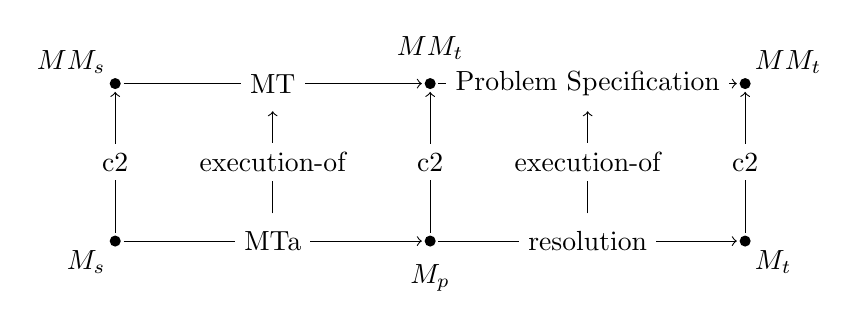
\begin{tikzpicture}
            \coordinate [label=-100:{$M_s$}]  (SM) at (0,0);
            \coordinate [label=100:{$MM_s$}]  (SMM) at (0,2);
            
            \coordinate [label={[label distance=5pt]-90:{$M_p$}}]  (PM) at (4,0); 
            \coordinate [label={[label distance=5pt]90:{$MM_t$}}]  (PMM) at (4,2);

            \coordinate [label=-10:{$M_t$}]  (TM) at (8,0);
            \coordinate [label=10:{$MM_t$}]  (TMM) at (8,2);

            \coordinate (S2P) at (2,0);
            \coordinate (SS2PP) at (2,2);
            \coordinate (P2T) at (6,0);
            \coordinate (PP2TT) at (6,2);
            
        
            \fill (SM) circle (2pt);
            \fill (TM) circle (2pt);
            \fill (SMM) circle (2pt);
            \fill (TMM) circle (2pt);
            \fill (PM) circle (2pt);
            \fill (PMM) circle (2pt);

          \draw[->, shorten <= 3pt, shorten >= 3pt] (SM) -- (PM) node [midway,fill=white] {MTa};
          \draw[->, shorten <= 3pt, shorten >= 3pt] (PM) -- (TM) node [midway,fill=white] {resolution};
          \draw[->, shorten <= 3pt, shorten >= 3pt] (PMM) -- (TMM) node [midway,fill=white] {Problem Specification};
          \draw[->, shorten <= 3pt, shorten >= 3pt] (SMM) -- (PMM) node [midway,fill=white] {MT};
          \draw[->, shorten <= 3pt, shorten >= 3pt,] (SM) -- (SMM) node [midway,fill=white] {c2};
          \draw[->, shorten <= 3pt, shorten >= 3pt] (TM) -- (TMM)node [midway,fill=white] {c2};
          \draw[->, shorten <= 3pt, shorten >= 3pt] (PM) -- (PMM)node [midway,fill=white] {c2};


            \draw[->, shorten <= 10pt, shorten >= 10pt,] (S2P) -- (SS2PP) node [midway,fill=white] {execution-of};
            \draw[->, shorten <= 10pt, shorten >= 10pt,] (P2T) -- (PP2TT) node [midway,fill=white] {execution-of};
        \end{tikzpicture}
            \caption{Two stage transformation, with first a standard transformation, followed by a problem resolution}
            \label{fig:MT+s}
        \end{figure}

        In \autoref{fig:MT+s} we have a sequence \autoref{fig:transfo} and \autoref{fig:search}. The source model is first transformed to a prototype model conforming to the target meta-model, which is subsequently transformed into a model satisfying the constraints.

        \subsubsection{Coupling Solvers with Model Transformations \cite{le_calvar_toward_2019,lecalvar_coupling_2021} \label{sssec:ATLc}}
        This effort is an extension to the ATL engine ATOL, which allows engineers to use OCL to not only make verifiable assertions about the models, but express constraint problems to be solved.
        
        Use-cases for this, illustrated by \autoref{fig:MT+s}, are when transforming to the provided target meta-models for JavaFX and Constraints, allowing for rapid development of applications based around graphical user interfaces. Users to define a meta-model and model for their application, and a transformation towards user-interface elements and constraints specifying desired positions for these elements.
        A first transformation from application model to JavaFX is performed, providing a prototype target model of which the attributes are refined using constraints.

        The constraint meta-model allows to create solver independent models, permitting the use a variety of solvers, such as Choco and Cassowary.
        
        % \begin{outline}
        %     \1 ATL + OCL
        %     \1 Constraint Solving of OCL
        %         \2 Constraint MM
        %         \2 Choco solver
        %         \2 Cassowary solver
        %     \1 ATL -> Endogenous/Exogenous Transformations
        %     \1 Constraints -> Endogenous Transformations
        %         \2 conforming to OCL and Constraint MM
        %         \2 Satisfiability
        %         \2 Optimality
        % \end{outline}
        % Transformations Endo/Exogenous + Search is Endogenous

                \begin{figure}
                \centering
                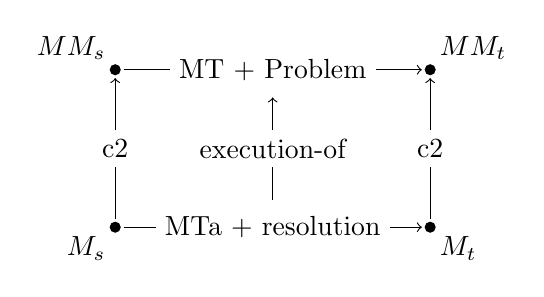
\begin{tikzpicture}
              \coordinate [label=-100:{$M_s$}]  (SM) at (0,0);
              \coordinate [label=-80:{$M_t$}] (TM) at (4,0);
              \coordinate (M2M) at (2,0);
            
              \coordinate [label=100:{$MM_s$}]  (SMM) at (0,2);
              \coordinate [label=80:{$MM_t$}]  (TMM) at (4,2);
              \coordinate (MM2MM) at (2,2);
            
                \fill (SM) circle (2pt);
                \fill (TM) circle (2pt);
                \fill (SMM) circle (2pt);
                \fill (TMM) circle (2pt);
              
              \draw[->, shorten <= 3pt, shorten >= 3pt] (SM) -- (TM) node [midway,fill=white] {MTa + resolution};
              \draw[->, shorten <= 3pt, shorten >= 3pt] (SMM) -- (TMM) node [midway,fill=white] {MT + Problem};
              \draw[->, shorten <= 3pt, shorten >= 3pt,] (SM) -- (SMM) node [midway,fill=white] {c2};
              \draw[->, shorten <= 3pt, shorten >= 3pt] (TM) -- (TMM)node [midway,fill=white] {c2};
            
                \draw[->, shorten <= 10pt, shorten >= 10pt,] (M2M) -- (MM2MM) node [midway,fill=white] {execution-of};
            \end{tikzpicture}
                \caption{Transformation and problem resolution performed as one execution}
                \label{fig:MTs}
            \end{figure}
        \vspace{-1em}
        In \autoref{fig:MTs} we see the merging of both steps in \autoref{fig:MT+s} into one. Both the transformation and problem specification are combined, and the combined specification is executed.

        \subsubsection{Transformations as logic problem}
        \label{sssec:logictransfo}
        In this sections we have two implementations of the logic solvers, first two efforts using Prolog to perform transformations and another implementing their own solver optimised for logic applied over models, and applying it to model transformations.   
        
        These two efforts, both using a Prolog Engine: both represent models, ensure their conformity, and perform transformations in the prolog language as facts and rules. \cite{schatz_design-space_2010,petter_solving_2009}
        However logical programming is able to express problems outside of model transformation, and thus can be used to express additional properties of the target model and transformation.
        These additional properties can be geometric constraints as in the example of \cite{petter_solving_2009}. 

        An issue for MDE is allowing domain experts to model, and to subsequently transform those models for other domain experts. And prolog and logical programming isn't the best candidate modeling language for modelers. \cite{petter_solving_2009} adds a layer allowing users to use MDE standards such as MOF, QVT, and OCL to declare models, transformations and constraints.
        
        % \subsubsection{QVTc \cite{petter_solving_2009}}
        % \begin{outline}
        %     \1 QVT + OCL (geometric)
        %     \1 Solving Constraints
        %         \2 Prolog Transformation
        %     \1 QVT + OCL Transformation definition
        %     \1 translated into prolog transformation
        % \end{outline}
        % \subsubsection{DSE \cite{schatz_design-space_2010}}
        % \begin{outline}
        %     \1 prolog transformation
        %         \2 MMM = prolog
        %         \2 M = prolog fact
        % \end{outline}

        % \subsubsection{Dynamic CSP over models \label{sssec:CSPM}}\cite{horvath_dynamic_2012}

        Another solution to the layer above logic programming, connecting to MDE technologies is proposed in \cite{horvath_dynamic_2012} where the models, transformations, and constraints are specified using the Viatra graph transformations language.
        This solution however also uses their own logic solver specialised in constraints over models, CSP(M).
        % This leverages logic solving techniques which 
        % \begin{outline}
        %     \1 both models and FOL constrains are expressed as graphs
        %     \1 Viatra
        %     \1 CSP(M)
        %         \2 Their own solver
        %         \2 backtracking
        %         \2 petri net abstraction
        % \end{outline}

        
        % \subsection{Transformation by Reinforcement // Improving / Reinforcing Transformations}
        \subsection{Learning Rule Application}
        \label{ssec:learnguard}

        % Engineering Context: Transformations are designed by engineers and AI finds optimal application of rules to acheive goal.

        Another augmentation AIs can provide model transformations, is learning when to apply transformation rules; Some transformations might propose small number of rules which have to be repeatedly applied to progress towards the target, or a large number of rules of which a subset achieves the desired goals.
        This can have the effect of encoding decision problems into the transformation specification. 
        % passing note: \cite{petter_solving_2009} uses choco so schedule the rules, which subsequently are performed by the "Prolog AI".

        % \begin{outline}
        %     \1 interative in nature
        %     \1 thus mainly endogenous transformation
        % \end{outline}


        \begin{figure}
            \centering
            \begin{minipage}[t]{.45\textwidth}
                \centering
                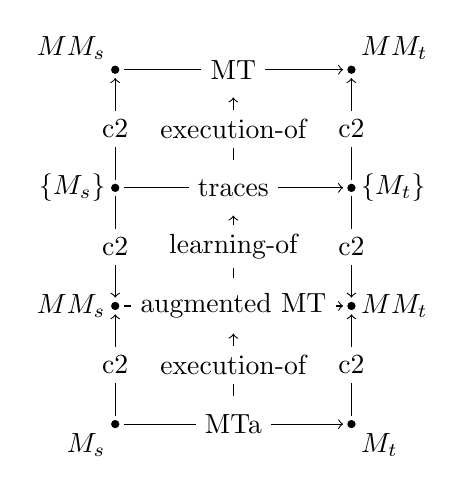
\begin{tikzpicture}[scale=.75]
                    \coordinate [label=-100:{$M_s$}]  (SM) at (0,0);
                    \coordinate [label=-80:{$M_t$}] (TM) at (4,0);
                        \coordinate (M2M) at (2,0);
                    
                    \coordinate [label=180:{$MM_s$}]  (SMM) at (0,2);
                    \coordinate [label=0:{$MM_t$}]  (TMM) at (4,2);
                        \coordinate (MM2MM) at (2,2);
                    
                    \coordinate [label=180:{$\{M_s\}$}]  (SMs) at (0,4);
                    \coordinate [label=0:{$\{M_t\}$}]  (TMs) at (4,4);
                        \coordinate (Ms2Ms) at (2,4);
            
                    \coordinate [label=100:{$MM_s$}]  (SMMu) at (0,6);
                    \coordinate [label=80:{$MM_t$}]  (TMMu) at (4,6);
                        \coordinate (MMu2MMu) at (2,6);
            
                    
                    \fill (SM) circle (2pt);
                    \fill (TM) circle (2pt);
                    \fill (SMM) circle (2pt);
                    \fill (TMM) circle (2pt);
                    \fill (SMs) circle (2pt);
                    \fill (TMs) circle (2pt);
                    \fill (SMMu) circle (2pt);
                    \fill (TMMu) circle (2pt);
                    
            
                    \draw[->, shorten <= 3pt, shorten >= 3pt] (SM) -- (TM) node [midway,fill=white] {MTa};
                    \draw[->, shorten <= 3pt, shorten >= 3pt] (SMM) -- (TMM) node [midway,fill=white] {augmented MT};
                    \draw[->, shorten <= 3pt, shorten >= 3pt,] (SM) -- (SMM) node [midway,fill=white] {c2};
                    \draw[->, shorten <= 3pt, shorten >= 3pt] (TM) -- (TMM)node [midway,fill=white] {c2};
                    \draw[->, shorten <= 3pt, shorten >= 3pt,] (SMs) -- (SMM) node [midway,fill=white] {c2};
                    \draw[->, shorten <= 3pt, shorten >= 3pt] (TMs) -- (TMM)node [midway,fill=white] {c2};
                    \draw[->, shorten <= 3pt, shorten >= 3pt,] (SMs) -- (SMMu) node [midway,fill=white] {c2};
                    \draw[->, shorten <= 3pt, shorten >= 3pt] (TMs) -- (TMMu)node [midway,fill=white] {c2};
                    \draw[->, shorten <= 3pt, shorten >= 3pt] (SMMu) -- (TMMu) node [midway,fill=white] {MT};
                    
                    \draw[->, shorten <= 10pt, shorten >= 10pt,] (M2M) -- (MM2MM) node [midway,fill=white] {execution-of};        
                    \draw[->, shorten <= 10pt, shorten >= 10pt,] (Ms2Ms) -- (MMu2MMu) node [midway,fill=white] {execution-of};
                    \draw[->, shorten <= 3pt, shorten >= 3pt] (SMs) -- (TMs) node [midway,fill=white] {traces};
                    \draw[->, shorten <= 10pt, shorten >= 10pt,] (MM2MM) -- (Ms2Ms) node [midway,fill=white] {learning-of};
            
                \end{tikzpicture}
                \caption{Transformation augmented by Reinforcement Learning}
                \label{fig:reinforcement}
            \end{minipage}\hfill
            \begin{minipage}[t]{.45\textwidth}
                \centering
                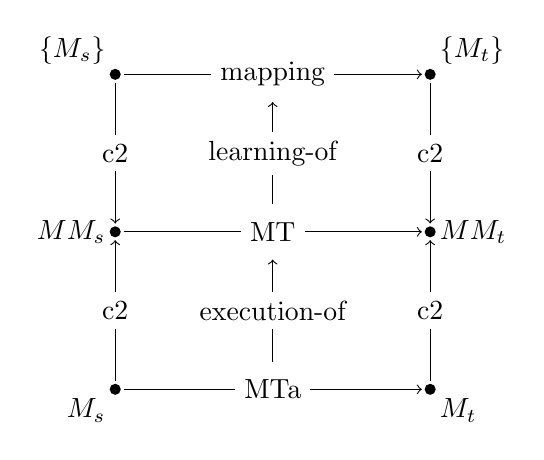
\begin{tikzpicture}
                    \coordinate [label=-100:{$M_s$}]  (SM) at (0,0);
                    \coordinate [label=-80:{$M_t$}] (TM) at (4,0);
                        \coordinate (M2M) at (2,0);
                    
                    \coordinate [label=180:{$MM_s$}]  (SMM) at (0,2);
                    \coordinate [label=0:{$MM_t$}]  (TMM) at (4,2);
                        \coordinate (MM2MM) at (2,2);
                    
                    \coordinate [label=100:{$\{M_s\}$}]  (SMs) at (0,4);
                    \coordinate [label=80:{$\{M_t\}$}]  (TMs) at (4,4);
                        \coordinate (Ms2Ms) at (2,4);
                    
                    \fill (SM) circle (2pt);
                    \fill (TM) circle (2pt);
                    \fill (SMM) circle (2pt);
                    \fill (TMM) circle (2pt);
                    \fill (SMs) circle (2pt);
                    \fill (TMs) circle (2pt);
            
                    \draw[->, shorten <= 3pt, shorten >= 3pt] (SM) -- (TM) node [midway,fill=white] {MTa};
                    \draw[->, shorten <= 3pt, shorten >= 3pt] (SMM) -- (TMM) node [midway,fill=white] {MT};
                    \draw[->, shorten <= 3pt, shorten >= 3pt,] (SM) -- (SMM) node [midway,fill=white] {c2};
                    \draw[->, shorten <= 3pt, shorten >= 3pt] (TM) -- (TMM)node [midway,fill=white] {c2};
                    \draw[->, shorten <= 3pt, shorten >= 3pt,] (SMs) -- (SMM) node [midway,fill=white] {c2};
                    \draw[->, shorten <= 3pt, shorten >= 3pt] (TMs) -- (TMM)node [midway,fill=white] {c2};
                    
                    \draw[->, shorten <= 10pt, shorten >= 10pt,] (M2M) -- (MM2MM) node [midway,fill=white] {execution-of};
                    \draw[->, shorten <= 3pt, shorten >= 3pt] (SMs) -- (TMs) node [midway,fill=white] {mapping};
                    \draw[->, shorten <= 10pt, shorten >= 10pt,] (MM2MM) -- (Ms2Ms) node [midway,fill=white] {learning-of};
            
                \end{tikzpicture}
                \caption{Transformation learned from examples}
                \label{fig:example}
                
            \end{minipage}
        \end{figure}

        \autoref{fig:reinforcement} shows us three distinct groups of source and target artefacts. The source and target meta-models represented each twice, source and target execution examples, and the final source and target models.
        Between the source and target elements we have transformation-likes, most importantly an initial transformation specification $MT$, and a final augmented specification. the initial (or intermediate) specifications are executed over sets of examples $\{M_s\}$ and $\{M_t\}$, and from the traces left by those executions improvements for the MT can be learnt. The final execution $MTa$ performs the task of producing the target $M_t$ from the source $M_s$.

        This figure shows a general case where source and target meta-models can be different, but most of the examples listed here perform and evaluate over sequences of transformations within a single meta-model, which allows to create optimising transformations.

        \subsubsection{Sequencing Transformation Rules~\cite{fatiregun_search_2003,fatiregun_evolving_2004,cooper_optimizing_1999,kulkarni_fast_nodate}}

        These first examples, tackle the use case of optimising code during compilation towards embedded systems. In this stage of optimisation, the program code is transformed to better suit the objectives. 
        Programs and programming languages are similar concepts to models and meta-models, and share a similar conformity relation, but are distinct in their technical spaces.
        The optimisation of the code can be done by a collection of algorithms, in our context transformations, performing actions such as removing variables, refactoring functions, numbering global values, register coalescing, etc... \cite{cooper_optimizing_1999} 
        The order in which these transformations are performed can have a significant impact on the desired qualities of the code, such as code size, as such AI techniques are employed to determine the best sequence of operation for the transformation.

        To use genetic algorithms, the order of operations is encoded into a genome, and a population of varying orders compete to produce the optimal code. The most successful orders, are mutated and combined with other successful orders, and the population is tested again, until a suitable order is found. 
        
        % \begin{outline}
        %     \1 Program Transformation a generally optimisaton
        %     \1 within the same language
        %     \1 nearly all examples cited are GA

        %     \1 Transformation operations are optimisation processes during compilations
        %         \2 register coalescing \cite{cooper_optimizing_1999}
        %         \2 global value numbering
        %     \1 optimal transformation is the right sequence of transformations
        %         \2 code for embedded systems
        %         \2 minimal code space

        % \end{outline} 


        \subsubsection{Reinforcement Learning applied to Model Transformations}
        % \subsubsection{Towards Reinforcement Learning for In-Place Model Transformations \cite{eisenberg_towards_2021}}
        These efforts explore the applications for reinforcement learning in model transformations. In the context of simple transformation rules which can be repeatedly applied to a model in order to progress towards a desired target, Q-Learning provides a framework to learn the the value of each available transformation rule given the current state of the model.
        
        A simple use case which portrays these kinds of transformations, is that of Pacman \cite{eisenberg_towards_2021}. The meta-model is that of pacman games: describing walls, pacman, ghosts and food. The models each represent a state of a pacman game: a maze of walls, remaining food in position on the floor, ghosts at their positions, and the pacman at theirs. Transformations describe going from one game state, to the next, such as pacman moving into an adjacent square with food and eating it.
        The objective is of the transformations, at each step, is to approach a model of a victorious game, with no food on the floor.

        In this context, Q-learning allows the transformation to know which is the best rule to apply for a given model, and to chain those transformations to optimise the model.
        
        % \begin{outline}
        %     \1 Hensin Endogenous Transformations
        %     \1 hensin rules for a pacman
        %     \1 rewards for pacman progress
        %     \1 uses Q-Learning to learn expected reward values of rules 
        % \end{outline}


        % \subsubsection{Model Repair with Quality-Based Reinforcement Learning - 2020 \cite{ludovico_model_2020}}
        % \begin{outline}
        %     \1 EMF
        %         \2 retruns problems,
        %             \3 duplicate class
        %             \3 duplicate inherited attribute
        %     \1 Their tools is PARMOREL
        %         \2 Q-Learning T100
        % \end{outline}
        The use case of \cite{ludovico_model_2020} describes model repair, a specific kind of model transformation, which can result in the model's conformity to a meta-model, or an optimisation relating to the semantics of the model, such as constraints.
        Their transformations take the errors returned by EMF\footnote{Eclipse Modeling Framework} tools on models being created, finds transformation rules to apply to improve the model. 
        Each state represents a model with an error in focus, and each action an available repair operation for the error.
        Q-Learning is again a strong candidate to give value to the repairs done by transformation actions for a given state.


        \subsubsection{Selecting Transformation Rules to Apply}
        \cite{fleck_marrying_2015} stands out from the others in this section by allowing for exogenous transformations, and by performing a search for each transformation. The search this effort provides is that of which rules to apply, which again differs from previous examples, by encoding the application of a rule as a decision variable as opposed to it's position in the sequence or the expected return, furthermore allowing to use a sub-set of a larger number rules as opposed to multiple applications, encouraging the possibility for exogenous transformations.
        Having encoded rule application as decision variables and the transformation as an objective of a decision problem, the MOEA tool (using GA, PSO, etc..) is handed the responsibility of finding the correct set of rules to apply, allowing for the transformation.
        % \begin{outline}
        %     \1 \cite{fleck_marrying_2015}
        %     \1 Hensin rules
        %         \2 rule application is a decision variablw
        %     \1 application is an optimisation problem
        %         \2 objectives defined in Java returning objective value
        %         \2 or OCL asserts
        %         \2 MOEA framework
        %             \3 evolutionary algorithms
        %             \3 GA
        %             \3 PSO
        %         \2 MOMoT <- their tool which combines the tool
        % \end{outline}
        % \subsection{Existence of a Transformation}
        % \subsection{Optimality of a Transformation}

         \subsection{Transformation by Example}
         \label{ssec:learnexample}

        % Engineering Context: Have the whole transformation derived from examples.

        The efforts listed in these applications of AI to model transformation, all share a similar goal of performing transformations, leveraging data from previously transformed models, allowing the reuse of previous efforts, and lessening efforts to automate future transformations.
        However different approaches use techniques from all across AI research, from classical AI atop of logic, to state-of-the-art neural network designs.
        The resulting transformation specifications are just as varied, ranging from specifications in transformation languages such as ATL or JESS to instances of a neural network.
        
        \autoref{fig:example} describes a situation where a transformation specification $MT$ is derived from sets of example source $\{M_s\}$ and target $\{M_t\}$ models conforming to their respective meta-models $MM_s$ and $MM_t$, and a mapping between them. 
        This learned specification is then executed $MTa$ to transform new models $M_s$ into acceptable targets $M_t$.
        \subsubsection{Learning \emph{Black-Box} Transformations}
        % \subsubsection{An LSTM-Based NN Architecture for Model Transformations - 2019 \cite{burgueno_lstm-based_2019}}
        \cite{burgueno_lstm-based_2019} employs a neural network to perform the transformation, allowing to approximate \emph{black box} transformation specifications from examples of source models and their targets. 
        
        In this context we refer to the structure and the parameters of the neural network as a transformation specification, while the path of activation though the network caused by the input, resulting in activation at the output as an transformation application.
        This requires a transformation between classing modeling languages and vectorised representations which the AI can manipulate.
        The encoder neural network, takes a vectorised form of the model and transforms it to a model \emph{understood} by the neural network. The decoder then performs the opposite, taking the neural network's understanding of the source, and translating to a vectorised form of the target model.
        
        
    % \begin{outline}
    %     \1 one of the rare neural networks
    %         \2 LSTM is State of the Art (GPT)
    %     \1 The neural network is represented by the MT definition
    %     \1 The input and output layers, instantiated with values, represent vectorised source and target models
    % \end{outline}
% \mtodo{Paper leading up to this one}

        \subsubsection{Learning Transformations as a Logic Problem}
        % \subsubsection{Model Transformation By Example using Inductive Logic Programming \cite{balogh_model_2009}}
        In the previously explored transformations as logical problems in \autoref{sssec:logictransfo}, source models are defined as fact, and logical inference rules allow to prove facts representing the target. The engineer would give source models and transformation rules, to get targets models.
        With the ALEPH ILP system, the application of which is explored in \cite{balogh_model_2009} as an extension to the work in \cite{varro_model_2006}, from solely providing facts - about background knowledge accompanied with positive and negative facts about the targets - we can find hypothesis to explain to positive facts from our knowledge, while not proving the negative facts.

        In the context of model transformations, we can provide facts representing source and target models, and ask the ALEPH system to determine which logical inference rules can prove the target facts from the source facts, providing the logical transformation between them.
% \begin{outline}
%     \1 aleph ILP engine <---
%     \1 Viatra graph transformations
%         \2 mapping of source and trager models
%     \1 prolog
%         \2 starts with background knowledge
%         \2 positive facts
%         \2 negative facts (become constraints)
%     \1 algorithms to get some hypothetical prolog rules
%         \2 context analysis for source and target model
%         \2 learning negative constraints from
% \end{outline}

% \mtodo{There are papers from Varro leading up to this \cite{vavarro_model_2006}}


        % \subsubsection{Model Transformation By Example \cite{strommer_model_2008}}
        % \begin{outline}
            
        % \end{outline}

        \subsubsection{Learning Transformation Specifications \cite{faunes_generating_2012,faunes_genetic-programming_2013}}
        This effort tries to produce the code for transformations specifications (in JESS but applicable to others like ATL), using genetic programming. Like other genetic algorithms, this involves encoding the problem as a genome, however in this case the genome is the code, and the genetic operations guarantee that the derived programs are syntactically and semantically valid.
        Therefore one starts with example source and target models, a population random but correct transformation rules, and a function to compare models produced by the population of transformations and example desired targets. The result of the process, is a transformation, or collection of rules, in the target transformation specification language. 
        % \begin{outline}
        %     \1 traget -> transformation rules in JESS (ynot ATL)
        %     \1 initial pop of random (but correct) rules
        %     \1 user provides 
        %         \2 fitness functions (distance between output and desire)
        %         \2 source and target examples sets
        %             \3 traces not important <- goal
        %         \2 why to create and encode random pop of JESS rules
        % \end{outline}

        \subsubsection{Reusing Examples of Transformations~\cite{kessentini_model_2008,kessentini_generating_2010,kessentini_search-based_2012}}
        % \subsubsection{kessentini}\cite{kessentini_model_2008,kessentini_generating_2010,kessentini_search-based_2012}
        In these approaches, example source models and transformations are dissected, in hopes to find reusable elements when transforming new models.
        The resulting parts of source models, and the transformation rules applicable to those parts, are used to define the dimensions of a space representing the solutions to the problem of model transformations.
        This allows the use of local (PSO) and global (SA) search algorithms, which encode their solutions spatially. 


        
        % \begin{outline}
        %     \1 tries to reuse parts of previous transformations to perform new ones
        %     \1 Uses ILP for definitions
        %     \1 PSO and SA
        %         \2 widely applied algorithms
        %         \2 SAT, etc...
        %         \2 ILP can be translated to 
        % \end{outline}

        % \subsection{...}
        
    \section{Discussions}
    % \mttodo{introduce the objective of the section}
    The analysis we made in the previous section can be used as a guide to identify approaches that have not been yet explored. In following we show a few examples of possible outcomes, exemplifying new pattern combinations (5.1), new instances for existing patterns (5.2), or new words for our language (5.3).
    \label{sec:discussion}
%     \subsection{Summary of the patterns observed}


%     Three main kinds of augmentations to model transformation specifications were observed across all these papers.
%     \begin{itemize}
%         \item extending the specification language to include decision problems \autoref{ssec:spaceexploration}
%         \item learning increasingly nuanced conditions for rule application \autoref{ssec:learnguard}
%         \item learning transformations specifications and rules \autoref{ssec:learnexample}
%     \end{itemize}
    
%     \begin{table}[!h]
%     \centering
%     \begin{tabular}{|c|c|}
%     \hline
%         Patern & Papers\\
%     \hline
%         \autoref{fig:MT+s} \autoref{fig:MTs} & \cite{lecalvar_coupling_2021,le_calvar_toward_2019} \cite{schatz_design-space_2010,petter_solving_2009,horvath_dynamic_2012}\\
%     \hline
%         \autoref{fig:reinforcement} & \cite{eisenberg_towards_2021,ludovico_model_2020,fatiregun_search_2003,fatiregun_evolving_2004,cooper_optimizing_1999,kulkarni_fast_nodate,fleck_marrying_2015}\\
%     \hline
%         \autoref{fig:example} & \cite{balogh_model_2009,burgueno_lstm-based_2019,faunes_generating_2012,faunes_genetic-programming_2013,kessentini_generating_2010,varro_model_2006,kessentini_model_2008,kessentini_search-based_2012,kessentini_generating_2010} \\
%     \hline
%     \end{tabular}
%     \caption{summary table of pattern to paper associations}
%     \label{tab:pap2pat}
% \end{table}

%         \begin{table}[!h]
%     \centering
%     \begin{tabular}{|c|c|}
%     \hline
%         Survey & Papers\\
%     \hline
%         \cite{boussaid_survey_2017} & \cite{fatiregun_evolving_2004,kulkarni_fast_nodate,faunes_generating_2012,kessentini_generating_2010,faunes_genetic-programming_2013,fleck_marrying_2015,kessentini_model_2008,cooper_optimizing_1999,fatiregun_search_2003,kessentini_search-based_2012} \\
%     \hline
%         \cite{kappel_model_2012} & \cite{kessentini_model_2008,varro_model_2006,balogh_model_2009}\\
%     \hline
%         X & \cite{eisenberg_towards_2021,burgueno_lstm-based_2019,le_calvar_toward_2019,petter_solving_2009,lecalvar_coupling_2021,horvath_dynamic_2012}\\
%     \hline
%     \end{tabular}
%     \caption{summary table of survey to paper associations}
%     \label{tab:pap2servey}
% \end{table}

    \subsection{Reusing Learned Transformations}
    While we have seen approaches for learning transformations (e.g. according to the pattern in \autoref{fig:example}), we have not observed tools that focus on reusing learned transformations for transforming different source and/or target metamodels. E.g., in \autoref{fig:reuse-example} we can see the pattern for a possible approach for reuse. A traditional transformation engine is used in a prepossessing stage (prepMT), translating to the source metamodel of the learned transformation.
    \vspace{-1em}

    \begin{figure}
            \centering
            % \begin{minipage}[t]{.45\textwidth}
                \centering
                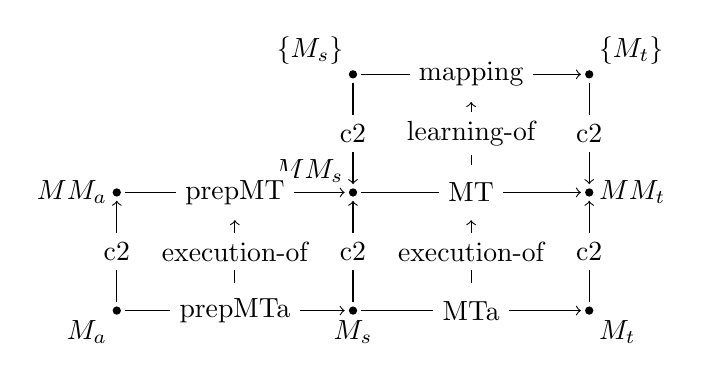
\begin{tikzpicture}[scale=.75]
                    \coordinate [label=-100:{$M_a$}]  (SSM) at (0,0);
                    \coordinate [label=180:{$MM_a$}]  (SSMM) at (0,2);
                        \coordinate (Ma2Ma) at (2,0);
                        \coordinate (MMa2MMa) at (2,2);
                
                    \coordinate [label=-90:{$M_s$}]  (SM) at (4,0);
                    \coordinate [label=-80:{$M_t$}] (TM) at (8,0);
                        \coordinate (M2M) at (6,0);
                    
                    \coordinate [label=150:{$MM_s$}]  (SMM) at (4,2);
                    \coordinate [label=0:{$MM_t$}]  (TMM) at (8,2);
                        \coordinate (MM2MM) at (6,2);
                    
                    \coordinate [label=100:{$\{M_s\}$}]  (SMs) at (4,4);
                    \coordinate [label=80:{$\{M_t\}$}]  (TMs) at (8,4);
                        \coordinate (Ms2Ms) at (6,4);


                    \fill (SSM) circle (2pt);
                    \fill (SSMM) circle (2pt);
                    \fill (SM) circle (2pt);
                    \fill (TM) circle (2pt);
                    \fill (SMM) circle (2pt);
                    \fill (TMM) circle (2pt);
                    \fill (SMs) circle (2pt);
                    \fill (TMs) circle (2pt);

                    \draw[->, shorten <= 3pt, shorten >= 3pt] (SSM) -- (SM) node [midway,fill=white] {prepMTa};
                    \draw[->, shorten <= 3pt, shorten >= 3pt] (SSMM) -- (SMM) node [midway,fill=white] {prepMT};
                    \draw[->, shorten <= 3pt, shorten >= 3pt,] (SSM) -- (SSMM) node [midway,fill=white] {c2};
            
                    \draw[->, shorten <= 3pt, shorten >= 3pt] (SM) -- (TM) node [midway,fill=white] {MTa};
                    \draw[->, shorten <= 3pt, shorten >= 3pt] (SMM) -- (TMM) node [midway,fill=white] {MT};
                    \draw[->, shorten <= 3pt, shorten >= 3pt,] (SM) -- (SMM) node [midway,fill=white] {c2};
                    \draw[->, shorten <= 3pt, shorten >= 3pt] (TM) -- (TMM)node [midway,fill=white] {c2};
                    \draw[->, shorten <= 3pt, shorten >= 3pt,] (SMs) -- (SMM) node [midway,fill=white] {c2};
                    \draw[->, shorten <= 3pt, shorten >= 3pt] (TMs) -- (TMM)node [midway,fill=white] {c2};

                    \draw[->, shorten <= 10pt, shorten >= 10pt,] (Ma2Ma) -- (MMa2MMa) node [midway,fill=white] {execution-of};
                    \draw[->, shorten <= 10pt, shorten >= 10pt,] (M2M) -- (MM2MM) node [midway,fill=white] {execution-of};
                    \draw[->, shorten <= 3pt, shorten >= 3pt] (SMs) -- (TMs) node [midway,fill=white] {mapping};
                    \draw[->, shorten <= 10pt, shorten >= 10pt,] (MM2MM) -- (Ms2Ms) node [midway,fill=white] {learning-of};
            
                \end{tikzpicture}
                \caption{Reusing transformation learned from examples}
                \label{fig:reuse-example}
            % \end{minipage}\hfill
            % \begin{minipage}[t]{.45\textwidth}
            %     \centering
            %     \begin{tikzpicture}[scale=.75]
            %         \coordinate [label=-100:{$M_s$}]  (SM) at (0,0);
            %         \coordinate [label=-80:{$M_t$}] (TM) at (4,0);
            %             \coordinate (M2M) at (2,0);
                    
            %         \coordinate [label=180:{$MM_s$}]  (SMM) at (0,2);
            %         \coordinate [label=0:{$MM_t$}]  (TMM) at (4,2);
            %             \coordinate (MM2MM) at (2,2);
                    
            %         \coordinate [label=180:{$\{M_s\}$}]  (SMs) at (0,4);
            %         \coordinate [label=0:{$\{M_t\}$}]  (TMs) at (4,4);
            %             \coordinate (Ms2Ms) at (2,4);
            
            %         \coordinate [label=100:{$MM_s$}]  (SMMu) at (0,6);
            %         \coordinate [label=80:{$MM_t$}]  (TMMu) at (4,6);
            %             \coordinate (MMu2MMu) at (2,6);
            
                    
            %         \fill (SM) circle (2pt);
            %         \fill (TM) circle (2pt);
            %         \fill (SMM) circle (2pt);
            %         \fill (TMM) circle (2pt);
            %         \fill (SMs) circle (2pt);
            %         \fill (TMs) circle (2pt);
            %         \fill (SMMu) circle (2pt);
            %         \fill (TMMu) circle (2pt);
                    
            
            %         \draw[->, shorten <= 3pt, shorten >= 3pt] (SM) -- (TM) node [midway,fill=white] {MTa};
            %         \draw[->, shorten <= 3pt, shorten >= 3pt] (SMM) -- (TMM) node [midway,fill=white] {augmented MT};
            %         \draw[->, shorten <= 3pt, shorten >= 3pt,] (SM) -- (SMM) node [midway,fill=white] {c2};
            %         \draw[->, shorten <= 3pt, shorten >= 3pt] (TM) -- (TMM)node [midway,fill=white] {c2};
            %         \draw[->, shorten <= 3pt, shorten >= 3pt,] (SMs) -- (SMM) node [midway,fill=white] {c2};
            %         \draw[->, shorten <= 3pt, shorten >= 3pt] (TMs) -- (TMM)node [midway,fill=white] {c2};
            %         \draw[->, shorten <= 3pt, shorten >= 3pt,] (SMs) -- (SMMu) node [midway,fill=white] {c2};
            %         \draw[->, shorten <= 3pt, shorten >= 3pt] (TMs) -- (TMMu)node [midway,fill=white] {c2};
            %         \draw[->, shorten <= 3pt, shorten >= 3pt] (SMMu) -- (TMMu) node [midway,fill=white] {MT};
                    
            %         \draw[->, shorten <= 10pt, shorten >= 10pt,] (M2M) -- (MM2MM) node [midway,fill=white] {execution-of};        
            %         \draw[->, shorten <= 10pt, shorten >= 10pt,] (Ms2Ms) -- (MMu2MMu) node [midway,fill=white] {execution-of};
            %         \draw[->, shorten <= 3pt, shorten >= 3pt] (SMs) -- (TMs) node [midway,fill=white] {traces};
            %         \draw[->, shorten <= 10pt, shorten >= 10pt,] (MM2MM) -- (Ms2Ms) node [midway,fill=white] {learning-of};
            
            %     \end{tikzpicture}
            %     \caption{Exogenous transformation augmented by Reinforcement Learning}
            %     \label{fig:exo-reinforcement}
                
            % \end{minipage}
        \end{figure}
        \vspace{-1em}

    \subsection{Exogenous Transformations by Searching for Sets of Rules}
    The example of using evolutionary techniques to search for a selection of rules to apply \cite{fleck_marrying_2015} suggests the ability to perform transformations between different meta-models and weaving meta-models.
    Other examples in the section sought to repeatedly apply rules as part of a sequence, meaning the target models must be very similar to their sources, in order for the same transformations to be repeatedly applied.
    When presenting \autoref{fig:reinforcement} this behaviour was alluded to; the figure describes a general case with independent source and target meta-models, however all examples collected limit themselves to endogenous transformations. 
    Selecting which rules to apply from a large set, or the combinations of rules from several specifications, would allow for a wide range of targets for a single specification.

    \subsection{Learning Constraint Problem Specifications for Model Transformations}
    % \mttodo{specification to specification learning}
    While several transformation approaches require users to write constraints, 
    %Model driven engineering aids in the communication between domain experts and engineers. MDE provides a framework for experts to express themselves clearly, translating to 
    writing a consistent and efficient constraint problem specification is non-trivial. Sometimes it is easier for domain experts to describe constraints using examples which do and don't satisfy them. In the field of constraints, there are efforts to derive conjectures \cite{beldiceanu_acquiring_2022} (a parallel to ALEPH's hypotheses) about data in the form of constraint problems.
    
    While learning deterministic transformations was observed, learning problem specifications observed augmenting transformations has not been. In the case of learning transformations as a logic problem \cite{balogh_model_2009}, the transformation was indeed able to be produced as a problem specification, but the use case didn't present the complexity of AI-augmented transformations.

    Hence, in our pattern language such component would require a new word, for Problem Learning (\autoref{fig:learnconstraint}), completing a set of 4 words describing all combinations of execution/learning of transformations/problem-specifications. 
    
    \vspace{-1em}
    % \mtodo{talk about what we excluded from our paper ?}
    
    % \mtodo{add table for all patterns shown in the paper, that will show that in this section we are just enumerating the missing combinations}
    
% \cite{kessentini_search-based_2012}
    % \subsection{Patterns outside the scope of this paper}
    % \subsubsection{Exogenous Augmented Transformations and choosing rule subsets}
    % \autoref{fig:reinforcement}
    % In all the examples of reinforcement learning applied to model transformations explored in this paper, all transformation were endogenous.
    % \mtodo{either choose a subset of rules, or set collection of few rules but duplicated}
    % \subsubsection{Learning Constraints} \autoref{fig:learnconstraint}
    \begin{figure}
                \centering
                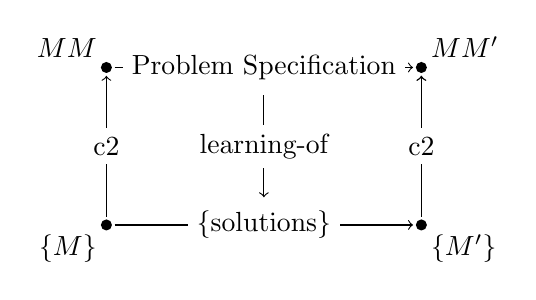
\begin{tikzpicture}
              \coordinate [label=100:{$MM$}]  (SMM) at (0,2);
              \coordinate [label=80:{$MM'$}] (TMM) at (4,2);
                \coordinate (MM2MM) at (2,2);
            
              \coordinate [label=-100:{$\{M\}$}]  (SM) at (0,0);
              \coordinate [label=-80:{$\{M'\}$}]  (TM) at (4,0);
                \coordinate (M2M) at (2,0);
            
                \fill (SM) circle (2pt);
                \fill (TM) circle (2pt);
                \fill (SMM) circle (2pt);
                \fill (TMM) circle (2pt);
              
              \draw[->, shorten <= 3pt, shorten >= 3pt] (SMM) -- (TMM) node [midway,fill=white] {Problem Specification};
              \draw[->, shorten <= 3pt, shorten >= 3pt] (SM) -- (TM) node [midway,fill=white] {\{solutions\}};
              \draw[->, shorten <= 3pt, shorten >= 3pt,] (SM) -- (SMM) node [midway,fill=white] {c2};
              \draw[->, shorten <= 3pt, shorten >= 3pt] (TM) -- (TMM)node [midway,fill=white] {c2};
              \draw[->, shorten <= 3pt, shorten >= 3pt] (TM) -- (TMM)node [midway,fill=white] {c2};
            
                \draw[->, shorten <= 10pt, shorten >= 10pt,] (MM2MM) -- (M2M) node [midway,fill=white] {learning-of};
            \end{tikzpicture}
                \caption{Problem Learning Pattern}
                \label{fig:learnconstraint}
                % \mttodo{there is no reference to this figure anymore in the text}
            \end{figure}

    % \mtodo{we are AI tool consumer not producers, so there is this pattern that is emerging in CSP. When it is ready we can use it}
    % \subsubsection{bidirectional transformations} \autoref{fig:bidir}
    %     \begin{figure}
    %             \centering
    %             \begin{tikzpicture}
    %           \coordinate [label=-100:{$M_s$}]  (SM) at (0,0);
    %           \coordinate [label=-80:{$M_t$}] (TM) at (4,0);
    %           \coordinate (M2M) at (2,0);
            
    %           \coordinate [label=100:{$MM_s$}]  (SMM) at (0,2);
    %           \coordinate [label=80:{$MM_t$}]  (TMM) at (4,2);
    %           \coordinate (MM2MM) at ( 2);
            
    %             \fill (SM) circle (2pt);
    %             \fill (TM) circle (2pt);
    %             \fill (SMM) circle (2pt);
    %             \fill (TMM) circle (2pt);
              
    %           \draw[<->, shorten <= 3pt, shorten >= 3pt] (SM) -- (TM) node [midway,fill=white] {MTa};
    %           \draw[->, shorten <= 3pt, shorten >= 3pt] (SMM) -- (TMM) node [midway,fill=white] {MT};
    %           \draw[->, shorten <= 3pt, shorten >= 3pt,] (SM) -- (SMM) node [midway,fill=white] {c2};
    %           \draw[->, shorten <= 3pt, shorten >= 3pt] (TM) -- (TMM)node [midway,fill=white] {c2};
            
    %             \draw[->, shorten <= 10pt, shorten >= 10pt,] (M2M) -- (MM2MM) node [midway,fill=white] {execution-of};
    %         \end{tikzpicture}
    %             \caption{Bidirectional Transformation}
    %             \label{fig:bidir}
    %         \end{figure}

    % \subsection{Optimising Problem Specifications augmenting transformations}
    % An important factor in the performance of problem resolutions is in fact the problem specification and tuning of the search.
    % How the problem is defined shapes the boundaries of the search space. Seemingly different solutions can also be symmetric, or trivially different, which can be quickly accounted for with the correct specification and use of the solver.
    % Notable problem types, or global constraints, have specific optimisations which can also be leveraged with adequate problem specification.

    % Benefiting from these performance boosts require a high level of nuance in the problem specification provided during transformations. OCL has been used in some examples, but doesn't provide the expressiveness of dedicated problem specification languages designed to be solved. 
    \vspace{-1em}
    \section{Conclusions and Future Work}
    \label{sec:conclusion}
    
%     \begin{outline}
%     \1 our plusvalu
%     \2 more general view than other surveys
%     \2 defini un language
%         \3 proposing patterns that don't exist
%     \1 reviews -> focus is on survey from a descriptive point of view
%     \1 globally how is the AI placed vs MT
%     \1 language to generalise existing and future usages
% \end{outline}

% \mttodo{the main objective is investigating how off-the-shelf AI is used in transformations, the language is only the means to do this}
    In this paper 
    we propose a classification of applications of AI in model transformations. To allow this we used a language of common patterns, based on existing mega-modeling languages, to represent AI operations in model transformations processes.
    %This paper offers a more general view than existing works which focused on specific kind of transformations or AI tools. 
    The language proposed allowed us to clearly form distinct categories for the use of AI in model transformations, 
    and we showed that a few simple patterns are sufficient to represent AI augmented model transformations found in the literature, revealing three main trends:  extending the specification language to include decision problems (\autoref{ssec:spaceexploration}), learning increasingly nuanced conditions for rule application (\autoref{ssec:learnguard}), learning transformations specifications and rules (\autoref{ssec:learnexample}).

    These patterns cover a wide set of applications of AI such as inferring model transformations, completing part of target models that cannot be easily computed by transformations or even replacing the transformation by a logic program.
     These different tasks can be organised in a few categories.
    We also identified possible patterns that have not been explored yet, such as problem learning for model transformation, and searching for exogenous rule application conditions.

    % \mtodo{what do we plan to do ? a more complete search and adding concepts if necessary ? should we go into details on how MT can include AI for its work}
    % \mtnote{In the future, we plan to further explore the literature, and this pattern language, verifying its coherence and ability to represent a larger number of AI applications in MT. Additionally, implementing our own application of AI in MT.}{some more interesting options may be using the language to define unexplored patterns, to define and maybe refactor transformation networks, to investigate conditions for tool replaceability}
    Future efforts on our behalf involve leveraging the pattern language to systematically explore the space of possible future AI usages, and to investigate conditions for tool replaceability and refactoring of transformation toolchains.
    
    
